\documentclass[11pt]{beamer}
\usetheme{Warsaw}
\usepackage[utf8]{inputenc}
\usepackage{amsmath}
\usepackage{amsfonts}
\usepackage{amssymb}
\usepackage{graphicx}
\usepackage{verbatim}
\usepackage{fancyvrb}
\usepackage{hyperref}
\usepackage{color}
\RecustomVerbatimCommand{\VerbatimInput}{VerbatimInput}{fontsize=\tiny}
\author{Jupiter Subgroup}
\title{Introduction to Making Documents with \LaTeX}

%\setbeamercovered{transparent} 
%\setbeamertemplate{navigation symbols}{} 
%\logo{} 
%\institute{} 
%\date{} 
%\subject{} 
\begin{document}

\begin{frame}
\titlepage
\end{frame}

%\begin{frame}
%\tableofcontents
%\end{frame}

%
%	Introduction
%
\begin{frame}{Introduction}
\begin{columns}
	\begin{column}{6cm}
		\underline{What \LaTeX{} is}
		\begin{itemize}
			\item	A cross-platform typesetting environment
			\item 	Best way to produce aesthetically pleasing, logically coherent documents, especially when dealing with mathematical equations
			\item 	Free and customizable
		\end{itemize}
	\end{column}
		\begin{column}{5cm}
		\underline{What \LaTeX{} isn't}
		\begin{itemize}
			\item WYSIWYG (What You See is What You Get)
				\begin{itemize}
					\item MS Word, LibreOffice
				\end{itemize}
			\item Bloated memory hog
		\end{itemize}
	\end{column}
	\end{columns}
\end{frame}

%
%	How it works
%
\begin{frame}{How it Works}
\begin{enumerate}
	\item The \TeX{} typesetting engine reads a plain text file, usually written using \LaTeX{} (a set of \TeX{} macros) \\
	\only<1>{\VerbatimInput{hello.tex}} 
	\item<2-> Produces a readable, formatted document image (.dvi) \\
		\only<2>{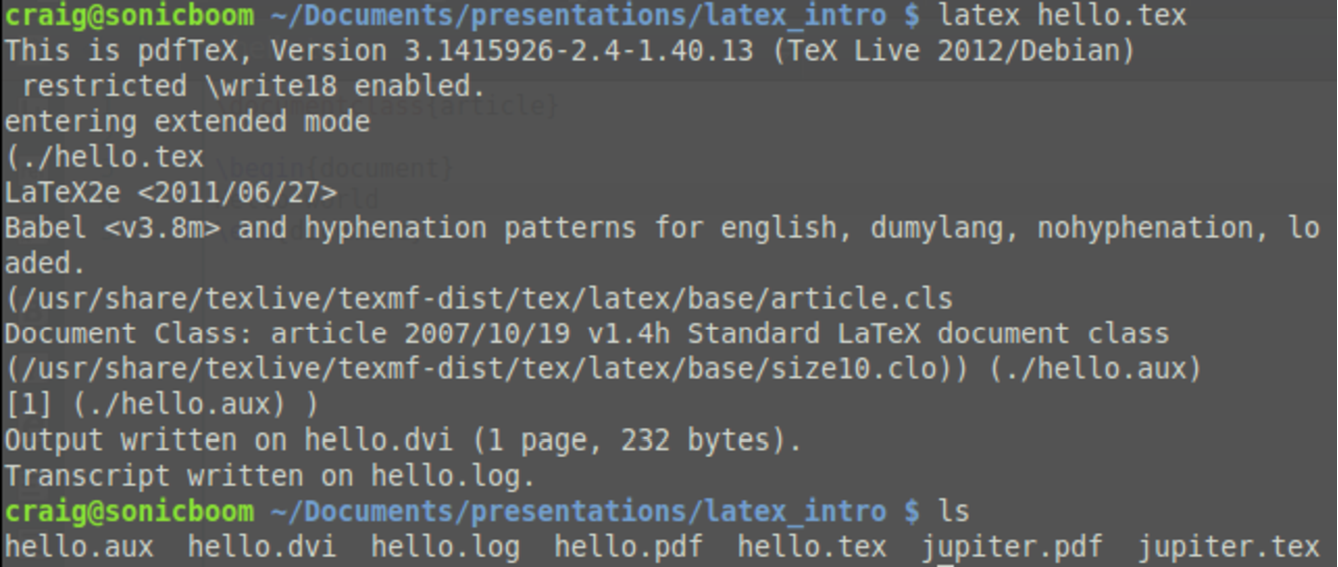
\includegraphics[scale=0.3]{hello_cli}}
	\item<3-> Convert to pdf (or straight to pdf using pdflatex)\\
			\only<3>{
\includegraphics[scale=.3]{hello}}
\end{enumerate}
\only<4> {Separates design from content $\rightarrow$ enhanced logical structure}
\end{frame}

%
%	What you need
%
\begin{frame}{What you Need}
\begin{enumerate}
	\item Text editor or IDE
	\begin{itemize}
		\item Texmaker, Vim/Emacs/gedit with plugins, Notepad++, Sublime
		\item Look for built-in output viewer, code completion \\
		\only<1>{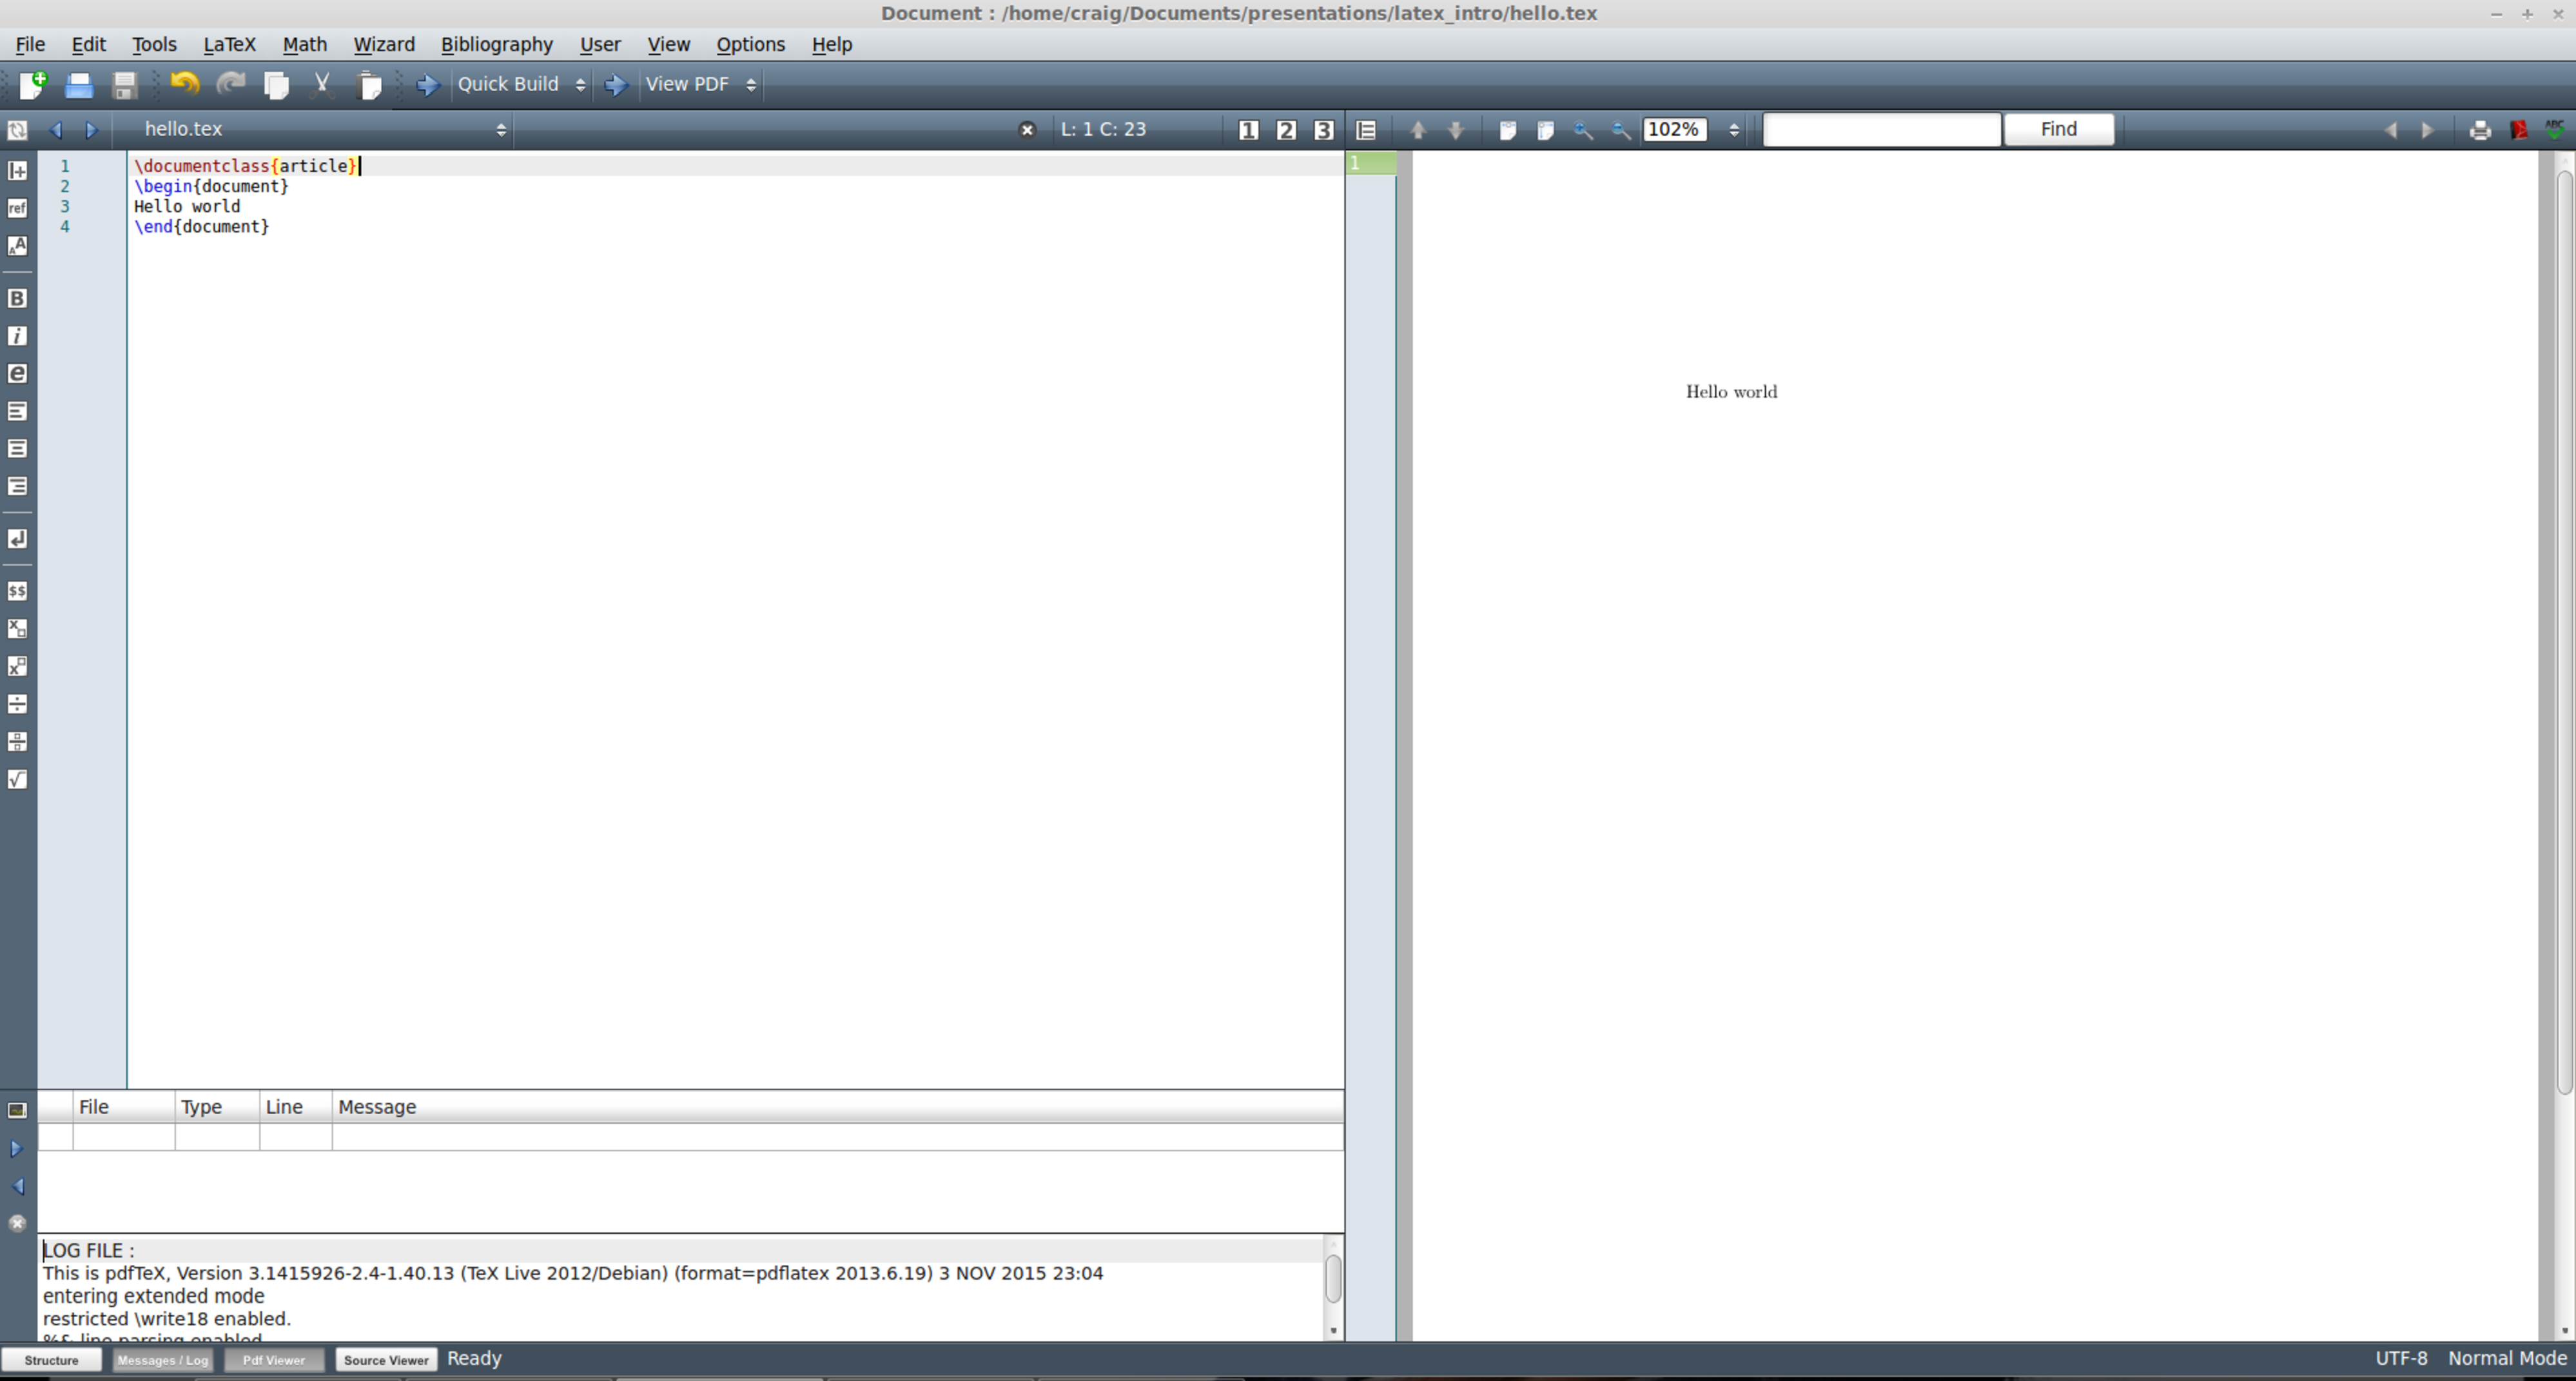
\includegraphics[scale=0.1]{texmaker}}
	\end{itemize}
	\item<2> Sane \LaTeX{} installation
	\begin{itemize}
		\item Windows - MikTeX
		\item Mac - MacTeX
		\item Linux - texlive
	\end{itemize}
\end{enumerate}
\end{frame}

%
% 	Special Characters
%
\begin{frame}{Special Characters, commands, and comments}
\begin{itemize}
	\item Special characters
	\begin{itemize}
		\item tells \LaTeX{} to do something, won't print like you intend
		\item \# \$ \% \^{} \& \_ \{ \} \~{}
\textbackslash
	\end{itemize}
	\item \LaTeX commands
	\begin{itemize}
		\item Start with a \textbackslash, i.e. \textbackslash backslash, \textbackslash alpha$\rightarrow \alpha$
	\end{itemize}
	\item Comment lines with \%
\end{itemize}
\end{frame}

%
% 	File Structure
%
\section{File Structure and Layout}
\begin{frame}{Input file structure and layout}
\begin{itemize}
	\item<1->	Preamble
	\begin{itemize}
		\item	Contains document type and all formatting directions and information not directly related to content
		\item Authors, date, institutions, title, external packages \\
		\only<1->{\VerbatimInput{header_example.tex}}
	\end{itemize}
	\item<2> \textbackslash begin\{document\} \ldots \textbackslash end\{document\}
\end{itemize}
\end{frame}

%
% 	Packages
%
\begin{frame}{Packages and external files}
\begin{itemize}
	\item Packages add customization and fine tuning
	\item Commonly used:
	\begin{itemize}
		\item amsmath -- must have for mathematical formulae
		\item geometry -- adjust page margins
		\item graphicx -- including images
		\item nag -- ensures up to date syntax
		\item cleverref -- manages references in a clever way
		\item hyperref -- functional document and hyperlinks
	\end{itemize}
	\item See: \href{http://www.howtotex.com/packages/9-essential-latex-packages-everyone-should-use/}{{\small \color{blue}{http://www.howtotex.com/packages/9-essential-latex-packages-everyone-should-use/}}}
\end{itemize}
\end{frame}

%
% 	Typesetting
%
\section{Typesetting}
\begin{frame}{Typesetting}
\begin{columns}
	\begin{column}[T]{0.6\textwidth}
		\begin{itemize}
			\item Paragraphs and sentences
			\begin{itemize}
			\scriptsize
				\item	paragraphs broken by empty line
				\item 	extra spaces after period ignored
				\item 	line break without new paragraph \textbackslash \textbackslash{} or \textbackslash newline
				\item \textbackslash \textbackslash* prohibits page break after new line
				\item \textbackslash newpage starts a new page
				\item be careful after equations 
			\end{itemize}
		\end{itemize}
	\end{column}
	\begin{column}[T]{6cm}
	\only<1>{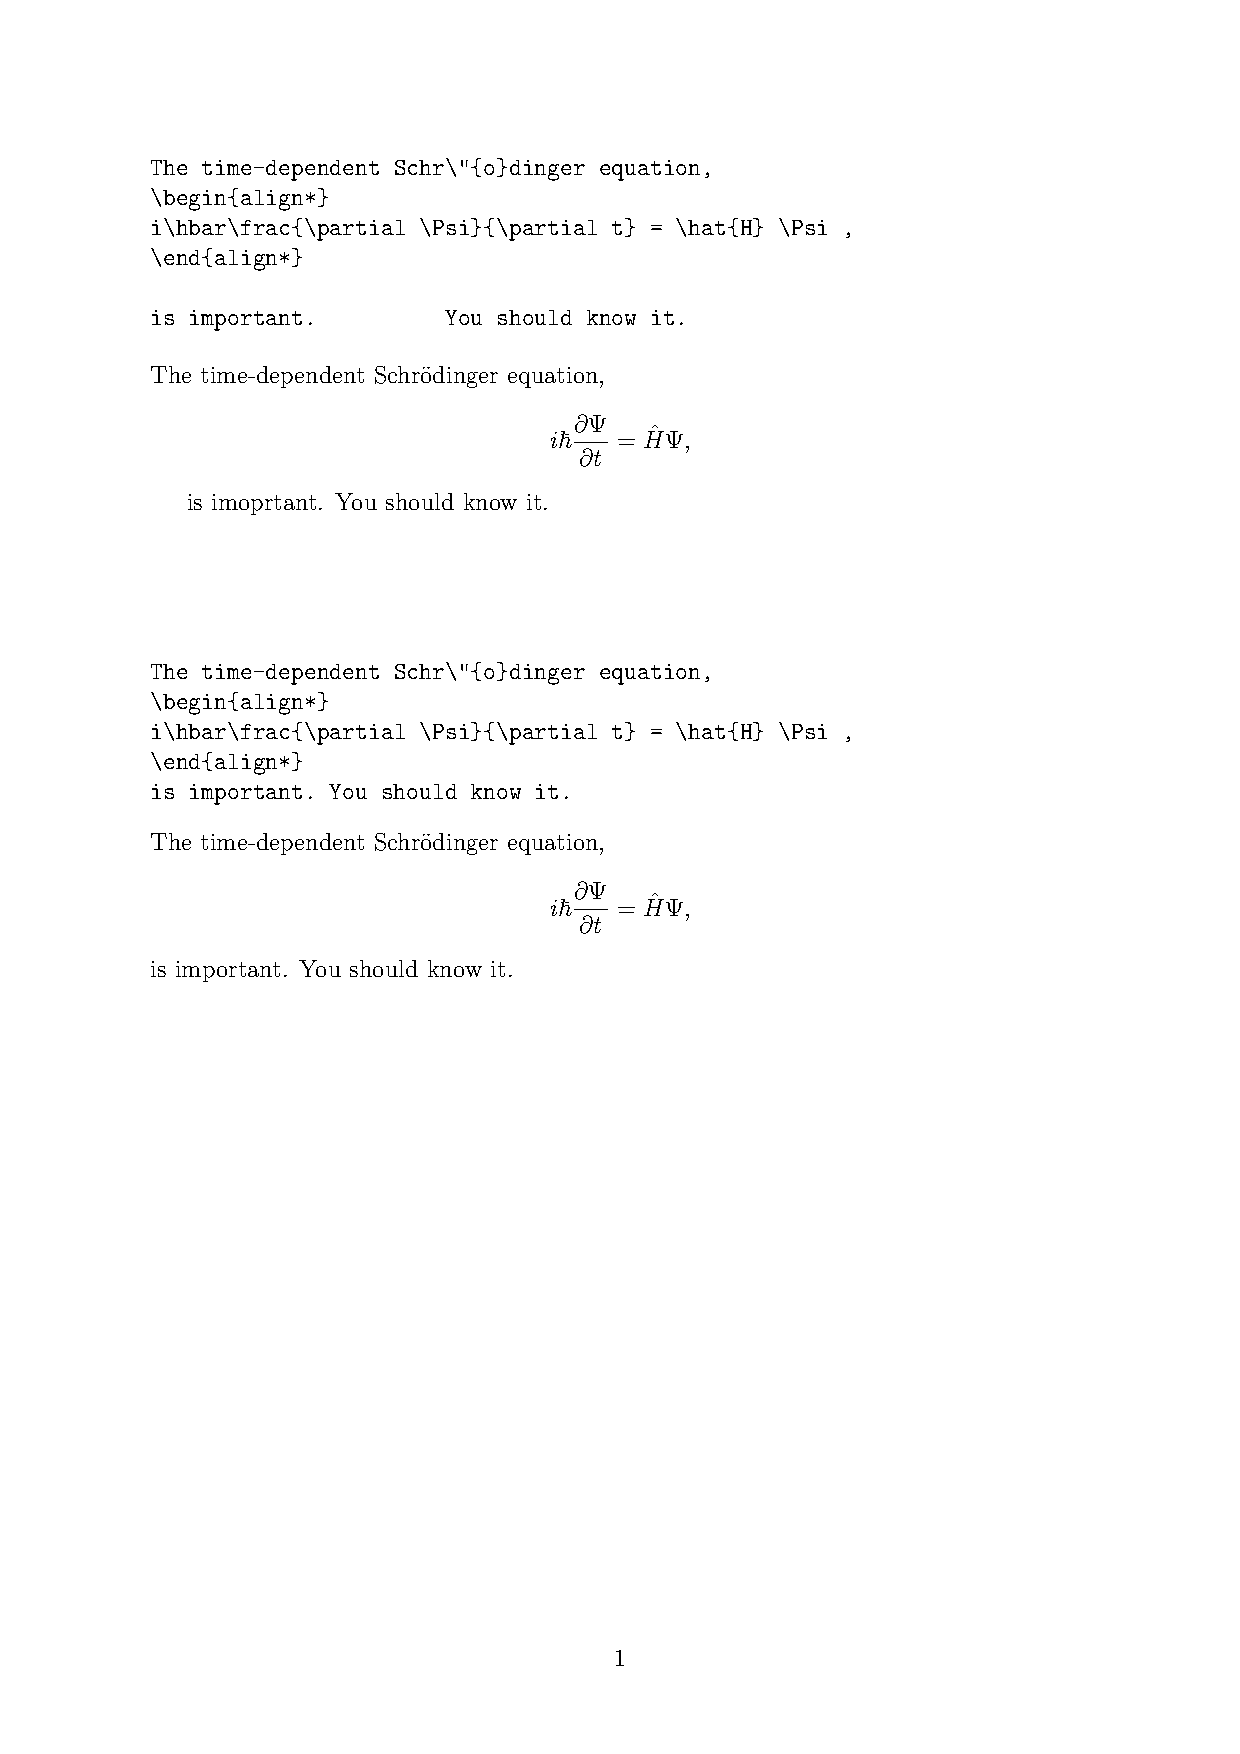
\includegraphics[scale=.4]{tdse-break}}
	\end{column}
\end{columns}
hyphenation, sections, chapters, alignment, itemize, enumerate, font sizes (table 6.3, 6.4)
\end{frame}

%Sections
\begin{frame}{Typesetting}
\begin{itemize}
	\item Organize content in outline form using Sections, subsections, chapters, and subchapters \\
	\only<1>{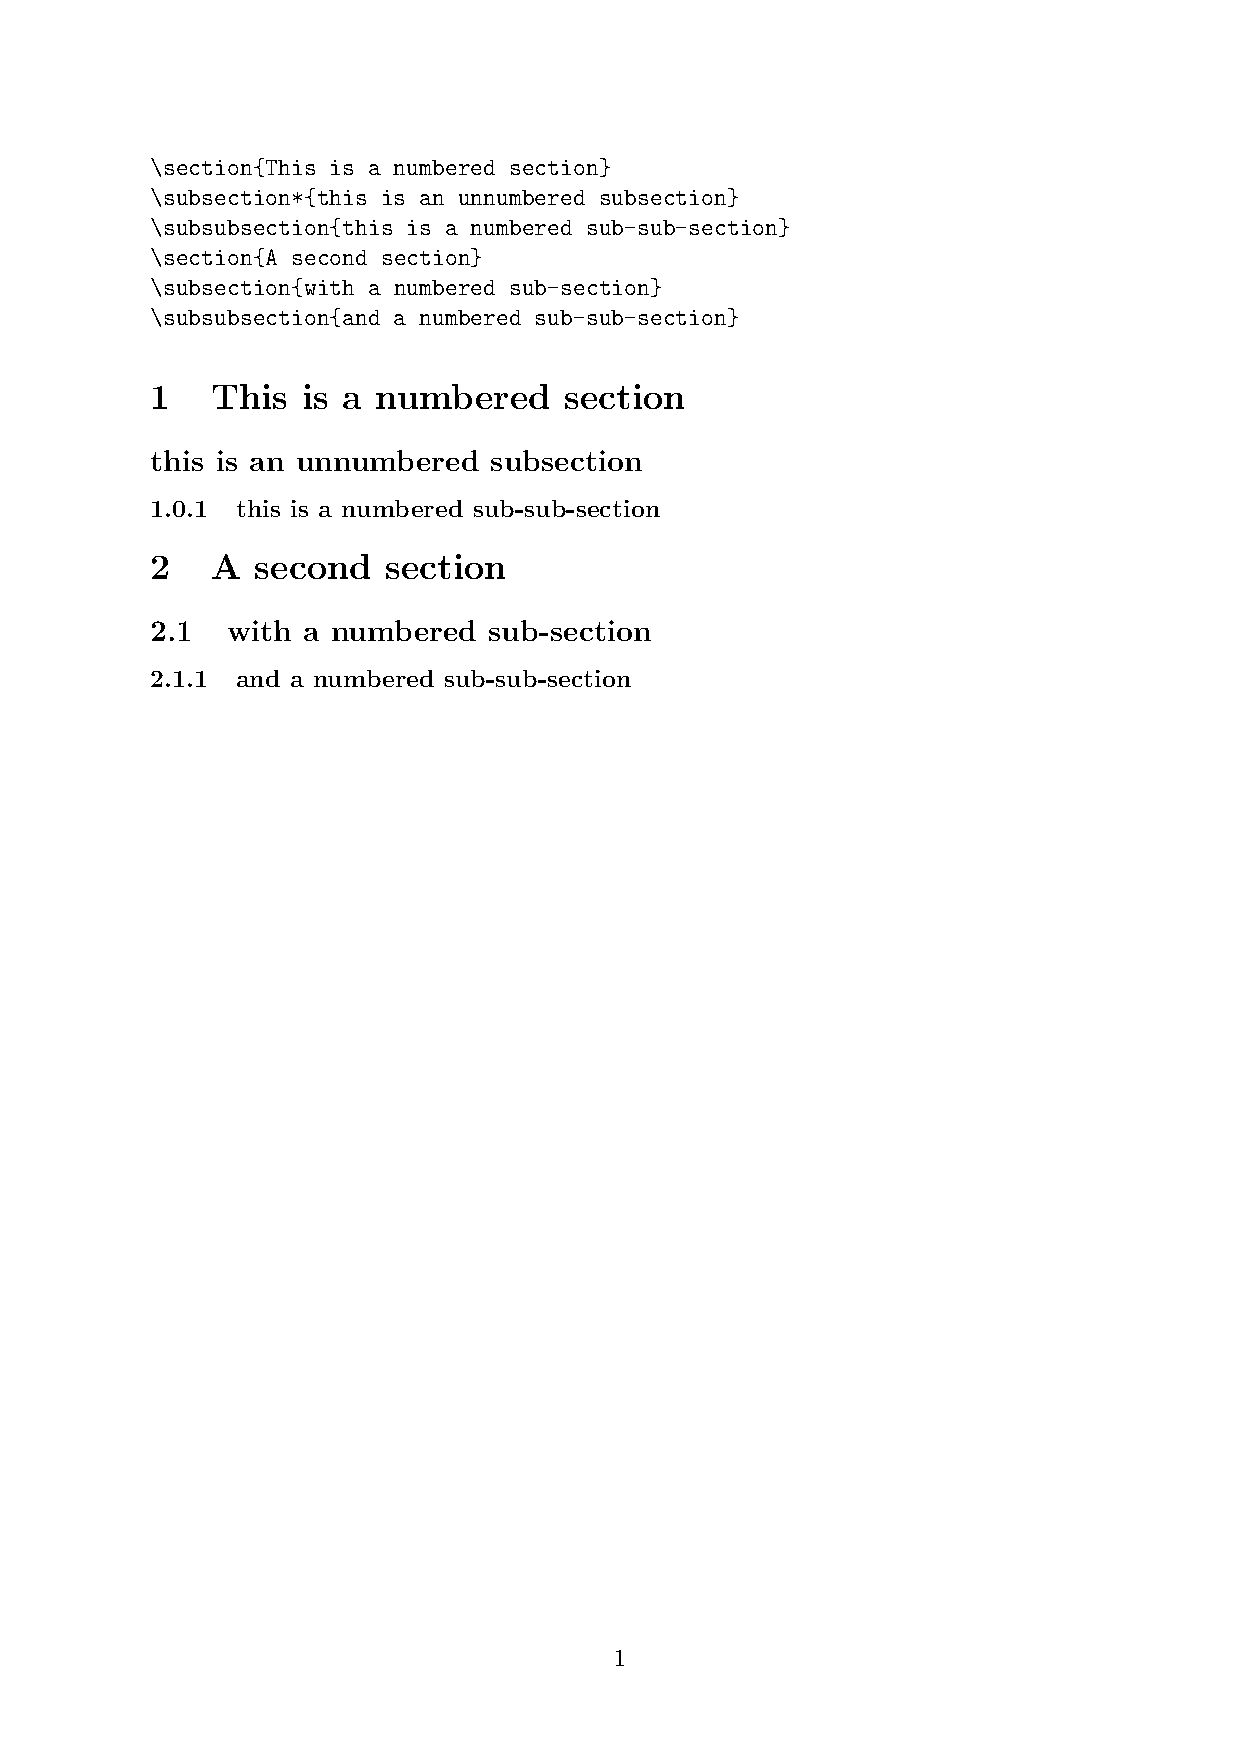
\includegraphics[scale=.4]{sections}}
\end{itemize}
\end{frame}

%Lists
\begin{frame}[fragile]\frametitle{Typesetting}
\begin{itemize}
	\item Make lists with ``itemize'' and ``enumerate'' environments \\
	\only<1>{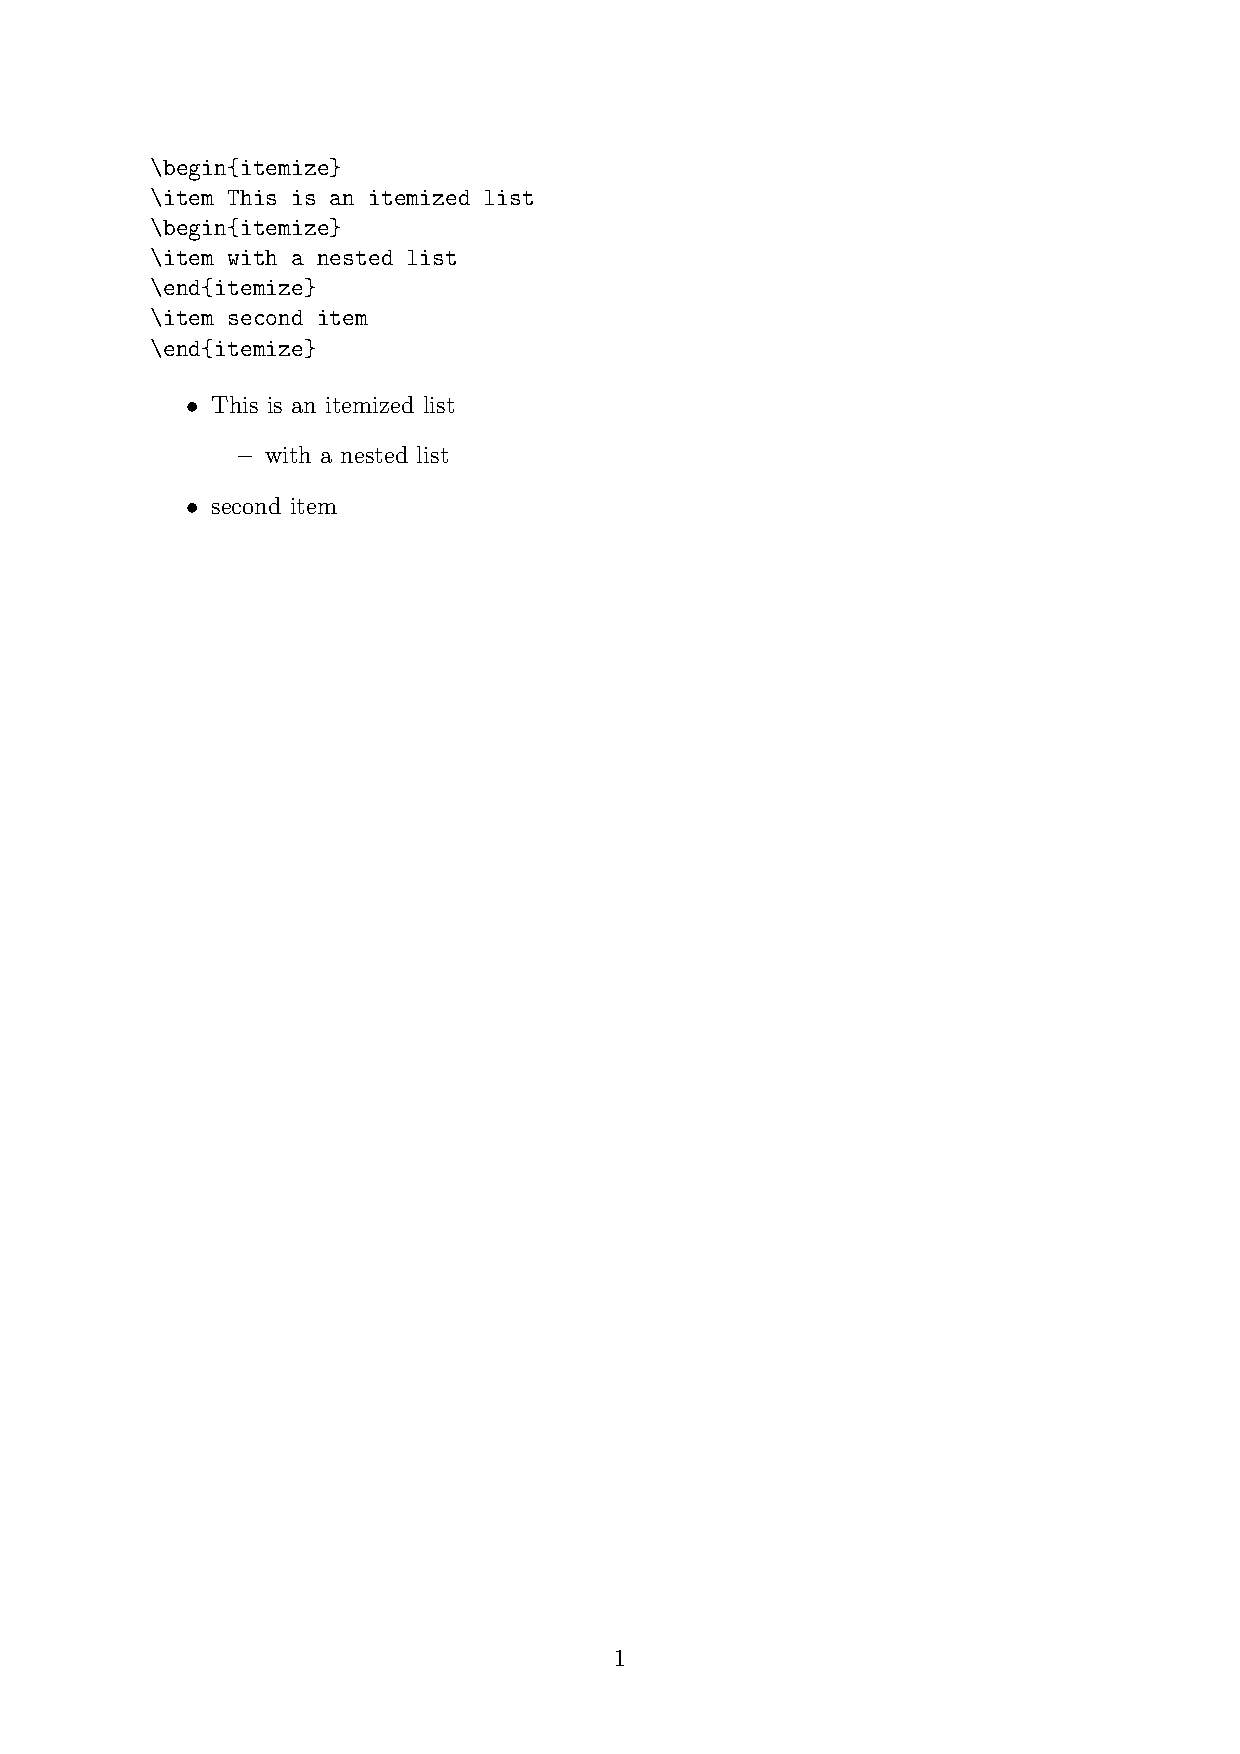
\includegraphics[scale=.4]{list1}}
	\only<2>{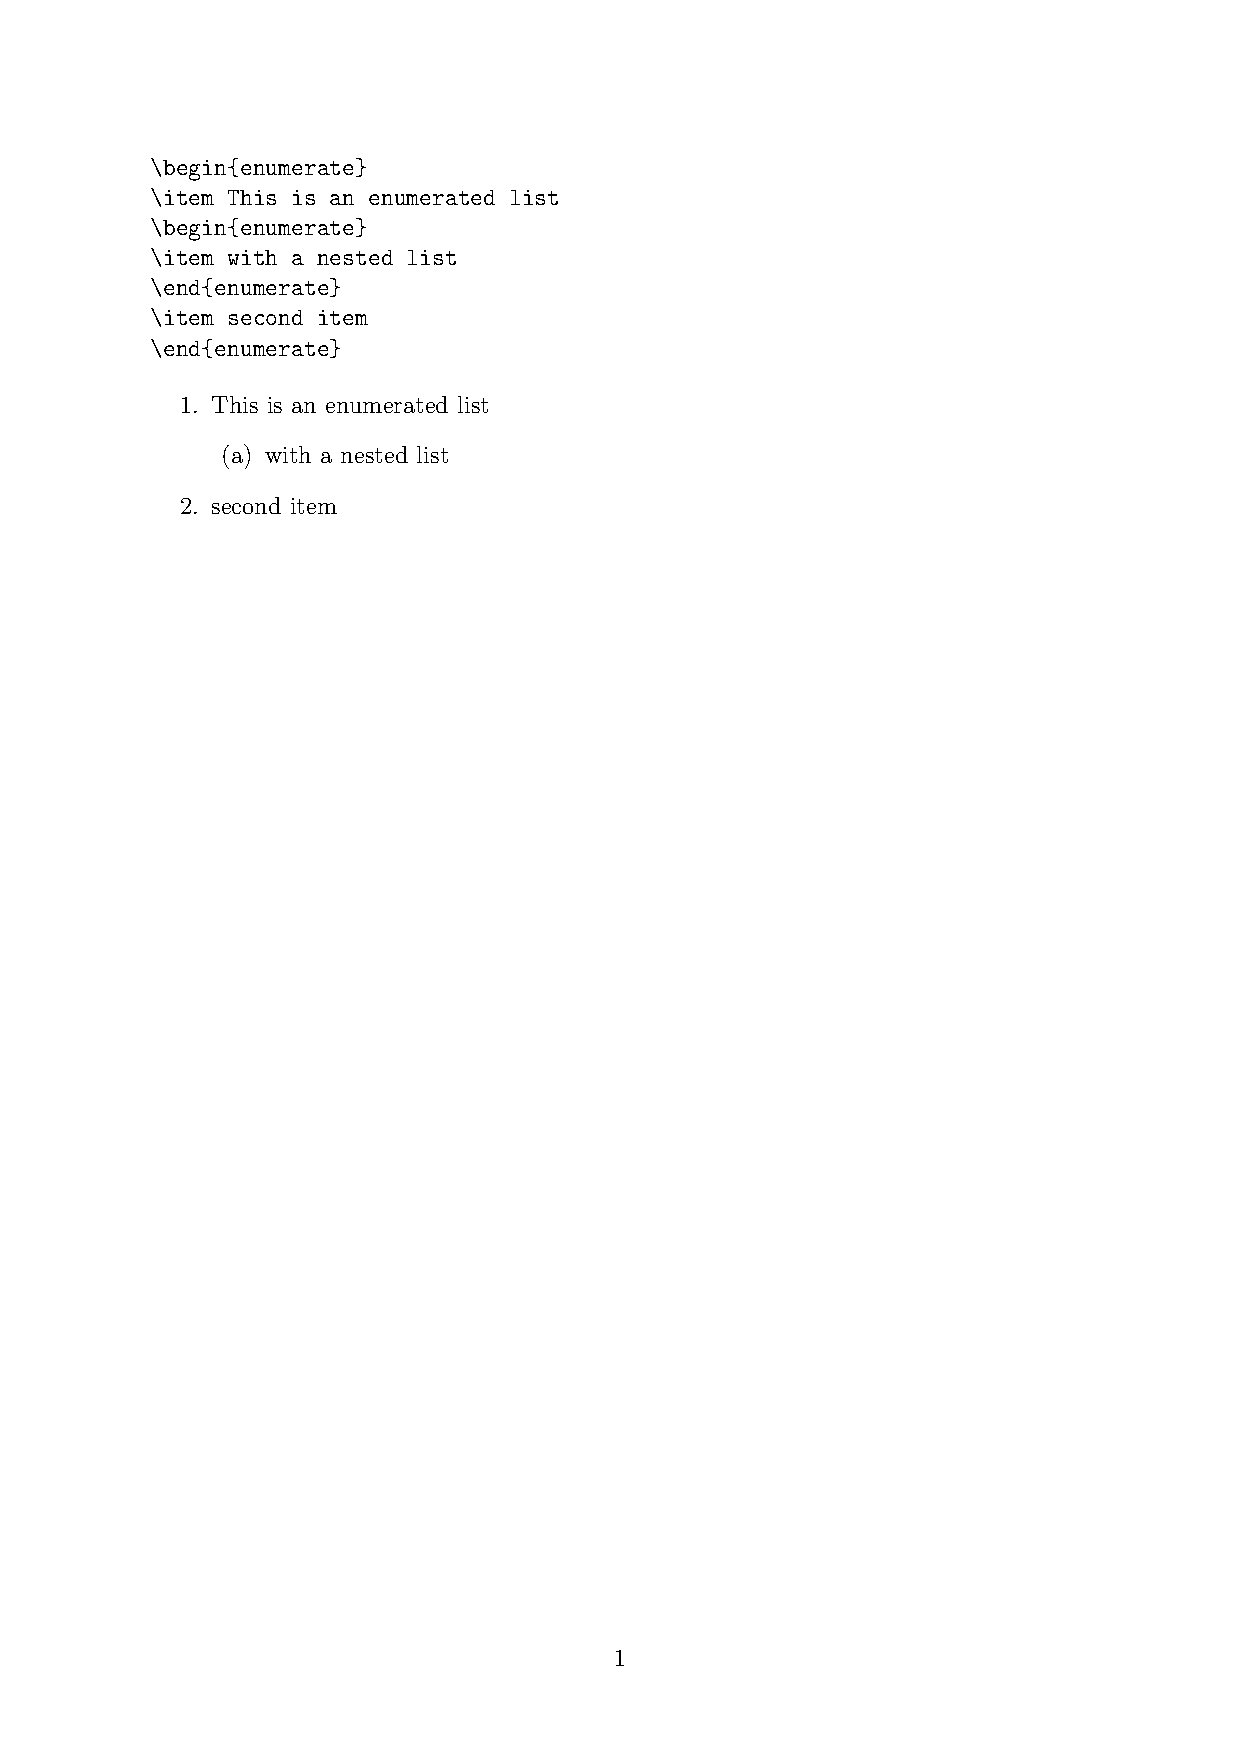
\includegraphics[scale=.4]{list2}}
	\begin{verbatim}
\begin{enumerate}
	\item This is an enumerated list
	\begin{enumerate}
			\item with a nested list
	\end{enumerate}
	\item second item
\end{enumerate}
\end{verbatim}
\begin{enumerate}
	\item This is an enumerated list
	\begin{enumerate}
			\item with a nested list
	\end{enumerate}
	\item second item
\end{enumerate}
\end{itemize}
\end{frame}

%
% 	File Structure
%
\begin{frame}[fragile]\frametitle{Some useful commands and characters}
\begin{itemize}
	\item bold, italic, underline
	\begin{itemize}
		\item \verb+\textbf{bold}+$\rightarrow$\textbf{bold}
		\item \verb+\textit{italic}+$\rightarrow$\textit{italic}, \verb+\emph{italic}+$\rightarrow$\emph{italic}
		\item \verb+\underline{underline}+$\rightarrow$\underline{underline}
	\end{itemize}
	\item other stuff
	\begin{itemize}
		\item superscript \verb+$^{...}$+ A$^{n}$
		\item subscript \verb+$_{...}$+ A$_{n}$
		\item degree  \verb+$^\circ$C+$\rightarrow^\circ$C
		\item quotation uses two grave accents (`) and two vertical quotation marks ('), ``A''
		\item Greek \verb+$\alpha_{\textrm{n}}^i$+ $\alpha_{\textrm{n}}^i$
	\end{itemize}
\end{itemize}
\end{frame}

%
% 	File Structure
%
\begin{frame}[fragile]\frametitle{Some useful environments}
\begin{itemize}
	\item<1-> \textbf{verbatim} -- direct quote, not interpreted
		\begin{itemize}
			\item Good for displaying code
			\item \verb+\usepackage{verbatim}+ and \verb+\usepackage{fancyvrb}+
			\begin{itemize}
				\item \verb+\begin{verbatim}...\end{verbatim}+
				\item \verb+\verb@...@+
				\item \verb+\VerbatimInput{hello.cc}+ \\ \VerbatimInput{hello.cc}
			\end{itemize}
		\end{itemize}
\end{itemize}
\end{frame}

\begin{frame}[fragile]\frametitle{Some useful environments}
\begin{itemize}
	\item<1-> \textbf{tabular} -- the way to make tables
		\begin{itemize}
			\item {\footnotesize \verb+\begin{tabular}[position]{table spec}...\end{tabular}+}
			\begin{itemize}
				\item 'position' specifies vertical position relative to surrounding text (t,b, or c)
				\item 'table spec' specifies number of columns and text justification (l,r, or c)
				\item \& moves to the next column, \verb+\\+ starts a new line, \verb+\hline+ inserts a horizontal line \\
				\begin{columns}
				\begin{column}{5cm}
					\VerbatimInput{table.tex}				
				\end{column}
				\begin{column}{5cm}
					\begin{tabular}{|r|l|}
					\hline
					7C0 & hexadecimal \\
					3700 & octal \\ \cline{2-2}
					11111000000 & binary \\
					\hline \hline
					1984 & decimal \\
					\hline
					\end{tabular}
				\end{column}
				\end{columns}
			\end{itemize}
		\end{itemize}
\end{itemize}
\end{frame}

%
% 	Types of formulae
%
\section{Mathematical Formulae}
\begin{frame}[fragile]\frametitle{Mathematical Formulae}
Producing consistent, aesthetically pleasing mathematical formulae is the main strength of \TeX
\begin{itemize}
	\item Use \verb+amsmath+ package, included with all installations
	\begin{itemize}
		\item \verb+\usepackage{amsmath}+
	\end{itemize}
	\item Produced by the American Mathematical Society
	\item Types of equations
	\begin{itemize}
		\item<2> inline -- This, $0.25+\frac{3}{4}=1$, is an inline equation
	\end{itemize}
\end{itemize}
\end{frame}

\begin{frame}[fragile]\frametitle{Mathematical Formulae}
Producing consistent, aesthetically pleasing mathematical formulae is the main strength of \TeX
\begin{itemize}
	\item Use \verb+amsmath+ package, included with all installations
	\begin{itemize}
		\item \verb+\usepackage{amsmath}+
	\end{itemize}
	\item Produced by the American Mathematical Society
	\item Types of equations
	\begin{itemize}
		\item displayed and numbered \\
			This is a displayed and numbered equation,
			\begin{align}
				0.25+\frac{3}{4}=1
			\end{align}
	\end{itemize}
\end{itemize}
\end{frame}

\begin{frame}[fragile]\frametitle{Mathematical Formulae}
Producing consistent, aesthetically pleasing mathematical formulae is the main strength of \TeX
\begin{itemize}
	\item Use \verb+amsmath+ package, included with all installations
	\begin{itemize}
		\item \verb+\usepackage{amsmath}+
	\end{itemize}
	\item Produced by the American Mathematical Society
	\item Types of equations
	\begin{itemize}
		\item displayed and unnumbered \\
			This is a displayed and unnumbered equation,
			\begin{align*}
				0.25+\frac{3}{4}=1
			\end{align*}
	\end{itemize}
\end{itemize}
\end{frame}

\begin{frame}[fragile]\frametitle{Mathematical Formulae}
Inline equations obtained from math mode with \verb+$...$+
\begin{itemize}
	\item Fractions are displayed differently, text is italicised
	\item reserve for less important formulae
\end{itemize}
\begin{columns}
\begin{column}{0.5\textwidth}
\VerbatimInput{inline.tex}
\end{column}
\begin{column}{0.5\textwidth}
Add $a$ squared and $b$ squared 
to get $c$ squared. Or, using 
a more mathematical approach: 
$a^2 + b^2 = c^2$ 
\end{column}
\end{columns}
\end{frame}

\begin{frame}[fragile]\frametitle{Mathematical Formulae}
Display equations with \verb+\begin{align}...\end{align}+
\begin{columns}
	\begin{column}{0.5\textwidth}
		\VerbatimInput{display.tex}
	\end{column}
	\begin{column}[T]{0.5\textwidth}
		Einstein says
		\begin{align}
			E = mc^2 
		\end{align}
		He didn’t say
		\begin{align}
			1 + 1 = 3 
		\end{align}
	\end{column}
\end{columns}
\only Equation numbers are tracked by a counter, can be manually set \verb+\setcounter{equation}{0}+ \setcounter{equation}{0}\\
\begin{align}
			E = mc^2 
		\end{align}
\end{frame}

\begin{frame}[fragile]\frametitle{Mathematical Formulae}
Display unnumbered equations with \verb+\begin{align*}...\end{align*}+
\begin{columns}
	\begin{column}{0.5\textwidth}
		\VerbatimInput{display-nonumbered.tex}
	\end{column}
	\begin{column}[T]{0.5\textwidth}
		Einstein says
		\begin{align*}
			E = mc^2 
		\end{align*}
		He didn’t say
		\begin{align*}
			1 + 1 = 3 
		\end{align*}
	\end{column}
\end{columns}
\end{frame}

\begin{frame}[fragile]\frametitle{Multi-line equations}
Use \verb+align+ environment for multi-line equations, align with \&. Use \verb+\nonumber+ to omit equation number on specific line
\begin{columns}
	\begin{column}{0.5\textwidth}
		\VerbatimInput{tdse-align.tex}
	\end{column}
	\begin{column}[T]{0.5\textwidth}
\begin{align}
	i\hbar\frac{\partial \Psi}{\partial t} = & \hat{H} \Psi \nonumber \\
	=& E \Psi
\end{align}
	\end{column}
\end{columns}
\end{frame}
%
% 	Useful commands
%
\begin{frame}[fragile]\frametitle{Some useful commands}
Greek
\begin{itemize}
	\item \verb+\alpha, \beta, gamma+ $\alpha, \beta, \gamma$ \\
	\item \verb+\varepsilon, \epsilon+ $\varepsilon, \epsilon$ \\
\end{itemize}
Sum, integral, product
\begin{columns}
	\begin{column}{0.5\textwidth}
		\VerbatimInput{sumintprod.tex}
	\end{column}
	\begin{column}[T]{0.5\textwidth}
\begin{align*}
\sum_{i=1}^n \qquad
\int_0^{\frac{\pi}{2}} \qquad
\prod_\epsilon
\end{align*}
	\end{column}
\end{columns}
\begin{itemize}
	\item \verb+\hat{H}+ $\hat{H}$
	\item \verb+\times+ A$\times$B, \verb+\cdot+ A$\cdot$B
	\item \verb+\partial+ $\partial$
\end{itemize}
Greek, super and sub script, sum (substack), integral, product operators, dots, frac, predefined functions, partial
\end{frame}

%
% 	Matrices
%
\begin{frame}{Arrays and matrices}
uses array environment for arrays, amsmath uses matrix environments
\end{frame}

%
% 	File Structure
%
\begin{frame}{Graphics}
use graphicx package (options), no real standard find what works, figure env. center, caption, includegraphics, remove extensions to avoid conflict b/w latex pdflatex
\end{frame}

%
% 	Bibliography
%
\begin{frame}{Bibliographies}
Use BibTeX, keep main bib file w/ consistent naming convention, bibliography command at end, bibliographystyle at beginning
\end{frame}

%
% 	Cross referencing
%
\begin{frame}{Cross referencing and citation}
Cleveref package, cite, ref, naming labels
\end{frame}

%
% 	Custom Commands
%
\begin{frame}{Custom commands}
newcommand-name, num of args, definition, hashtag w/ number for arguments, bra, ket, braket, 2x2 matrix \\
newenvironment, renewenvironment to override existing commands
\end{frame}

%
% 	Chemistry specific 
%
\begin{frame}{Chemistry specific packages}
https://www.ctan.org/topic/chemistry, chemfig-rings, rxn, achemso
\end{frame}

%
% 	Putting it all together
%
\begin{frame}{Putting it all together}
Keep a universal header, bib, and main document template. Copy and edit as needed. Example file with header, equations, cross reference, citations, and sections
\end{frame}

%
%	Resources
%
\begin{frame}{Resources}
lshort, ctan, http://www.xm1math.net/texmaker/
\end{frame}


\end{document}